\documentclass[conference]{IEEEtran}
\IEEEoverridecommandlockouts
% The preceding line is only needed to identify funding in the first footnote. If that is unneeded, please comment it out.
\usepackage{cite}
\usepackage{amsmath,amssymb,amsfonts}
\usepackage{algorithmic}
\usepackage{graphicx}
\usepackage{textcomp}
\usepackage{xcolor}
\def\BibTeX{{\rm B\kern-.05em{\sc i\kern-.025em b}\kern-.08em
    T\kern-.1667em\lower.7ex\hbox{E}\kern-.125emX}}
\begin{document}

\title{Balancing Image Compression and OCR Accuracy in Workflow Documentation}

\author{\IEEEauthorblockN{Matthew Feroz}
\IEEEauthorblockA{\textit{Department of Software Engineering}\\
\textit{Stevens Institute of Technology}\\
Hoboken, NJ, USA \\
Email: mferoz@stevens.edu}
}

\maketitle

\begin{abstract}
Modern knowledge work increasingly involves interacting with rich graphical interfaces such as code hosting platforms, issue trackers, spreadsheets, and game user interfaces. Much of the information needed for documentation and auditing exists only transiently on screen, so engineers often rely on screenshots and manual notes. Automating this process requires robust pipelines that can extract and interpret textual information from images under realistic quality constraints. Optical character recognition (OCR) performance, however, is highly sensitive to image compression, and the resulting textual feature space is typically high-dimensional and sparse. In this paper, we study how much JPEG compression can be applied to screenshots from four representative workflows---committing and pushing a GitHub change, creating a Jira ticket, copying data between spreadsheet tables, and interacting with a video game UI---before OCR becomes unreliable for downstream use. We define task-specific criteria for ``legible enough'' OCR based on the recovery of critical action text and evaluate a simple classifier on OCR outputs using three feature representations: raw bag-of-words, filtered bag-of-words, and TF--IDF. Our results characterize compression tolerance across workflows and illustrate how classical feature reduction techniques can mitigate the curse of dimensionality for documentation-oriented AI systems.
\end{abstract}

\begin{IEEEkeywords}
Optical character recognition, image compression, feature engineering, dimensionality reduction, documentation automation
\end{IEEEkeywords}

\section{Introduction}
Knowledge workers routinely interact with complex graphical user interfaces (GUIs) when committing code, filing issues, updating spreadsheets, or monitoring system state. The actions taken in these interfaces often need to be documented after the fact for auditing, compliance, or knowledge sharing. Today this documentation is largely manual: users capture screenshots and write natural language descriptions of what they did. This process is time-consuming, error-prone, and difficult to scale as workflows grow in complexity.

Automating documentation from screenshots requires two key capabilities. First, the system must reliably extract textual content from images using optical character recognition (OCR). Second, it must interpret that text to distinguish task-critical actions (e.g., ``Commit changes'', ``Create issue'', or specific cell updates) from background interface chrome. In practical deployments, screenshots may be aggressively compressed to save storage or bandwidth, especially when logging many interactions over time. This raises an important question for documentation-oriented AI systems: how much compression can be applied before OCR output becomes too degraded to support reliable downstream inference?

In addition to compression, there is a modeling challenge. Raw OCR outputs induce large, sparse feature spaces when represented as bag-of-words or n-grams. Learning on such high-dimensional data is susceptible to the curse of dimensionality and overfitting, particularly in small custom datasets. Modern deep learning architectures such as autoencoders and convolutional neural networks (CNNs) address this by learning compact internal representations, but simpler, classical feature engineering techniques can also provide effective dimensionality reduction.

In this work, we investigate these issues in the context of four concrete workflows: (1) committing and pushing a GitHub change, (2) creating a Jira ticket, (3) copying data between spreadsheet tables, and (4) interacting with a video game UI. For each workflow, we collect screenshots, generate multiple JPEG variants at different quality levels, and run OCR to obtain text. We then (i) determine, per workflow, the maximum compression level at which OCR remains ``legible enough'' for task-critical text, and (ii) construct a small labeled dataset of OCR snippets and evaluate a logistic regression classifier under three feature representations: raw bag-of-words, filtered bag-of-words, and TF--IDF-weighted features.

This paper makes three contributions. First, we propose a simple but practical framework for studying OCR robustness to JPEG compression in screen-based workflows. Second, we empirically examine how classical feature reduction techniques affect a downstream classifier that separates critical user actions from background text. Third, we connect these empirical findings to deep learning concepts such as autoencoders and CNNs, illustrating how manual feature engineering can approximate some of the benefits of learned latent representations.

\section{Related Work}
OCR robustness has been studied extensively in the context of scanned documents and natural scene text, where noise, blur, and low resolution can substantially degrade recognition accuracy. Prior work has investigated the impact of image quality factors such as contrast, resolution, and compression on OCR performance, typically using standardized datasets of scanned pages or photos. In contrast, our focus is on screenshots from interactive GUIs, where fonts are crisp but compression artifacts and small UI text can still pose challenges. This setting is increasingly important for documentation automation and robotic process automation (RPA), yet less explored in the literature.

Classical text representation methods for machine learning include bag-of-words (BOW) and n-gram models, where each unique token defines a feature dimension. These representations are simple and effective but can lead to extremely high-dimensional and sparse feature spaces, especially when applied to heterogeneous OCR outputs from multiple workflows. Term frequency--inverse document frequency (TF--IDF) weighting is a well-established technique for emphasizing discriminative terms by up-weighting tokens that are frequent in a document but rare across the corpus. Our work leverages these representations to study how dimensionality and feature weighting affect a simple classifier operating on OCR text.

Deep learning approaches have popularized learned representations that address the curse of dimensionality by compressing inputs into low-dimensional latent spaces. Autoencoders explicitly learn an encoder--decoder pair that maps high-dimensional inputs to compact codes and back, forcing the model to capture essential structure. CNNs, originally developed for images, reduce dimensionality through local receptive fields, weight sharing, and pooling operations, enabling scalable learning on high-resolution inputs. Although our experiments use linear models and explicit feature engineering, we interpret our findings through the lens of these architectures, viewing stop-word filtering and TF--IDF weighting as hand-crafted analogues of learned encoders that prioritize salient information.

\section{Methodology}
\subsection{Tasks and Data Collection}
We design four representative workflows to capture common patterns in screen-based knowledge work. The first workflow involves committing and pushing a change to a GitHub repository, highlighting developer tooling and version control. The second workflow focuses on creating a Jira ticket, representing issue tracking and project management. The third workflow captures copying structured data between spreadsheet tables, a frequent task in reporting and analysis. The fourth workflow uses a video game user interface as a non-business example, illustrating menus and heads-up display text.

For each workflow, we capture multiple full-screen or windowed screenshots showing the relevant user interface elements. Screenshots are saved as lossless PNG files, which we treat as our high-quality baselines. No pre-scanned documents are used; all images come from live web or application interfaces to better reflect modern usage scenarios. We then generate JPEG variants of each PNG at three aggressive quality levels (25, 5, and 1) using standard image encoding tools, keeping the resolution fixed. This yields a ``compression ladder'' for each screenshot that isolates the effect of JPEG quality. Quality level 5 was selected as the closest compression that remains readable by the human eye, while quality 1 represents the maximum possible JPEG compression (lowest quality setting) and approaches incomprehensibility (see Section~\ref{subsec:human-readability}). We use aggressive compression levels to ensure visible degradation even after post-processing that may occur in image viewers (see Section~\ref{sec:compression-selection}).

\subsection{OCR Pipeline and Legibility Criterion}
We apply an OCR engine to each image in the dataset, including both baseline PNGs and JPEG variants. For each workflow, we manually define a small set of task-critical textual elements, such as the ``Commit changes'' button label for GitHub, the ``Create'' button and field labels in Jira, key column headers and example cells in the spreadsheet, and menu or quest titles in the game UI. We consider OCR to be \emph{legible enough} at a given compression level if all task-critical phrases appear correctly, or with only minor, unambiguous typos, in the OCR output.

Using this definition, we record, for each workflow and each compression level, whether OCR succeeds or fails. This provides a direct operational answer to the question of how much compression can be applied before OCR becomes unusable for documentation of that workflow. In addition, we log the raw OCR text for selected images and compression levels to construct a small dataset for downstream classification experiments.

\subsection{Feature Engineering and Labeling}
From the collected OCR outputs, we build a labeled dataset of text snippets. Each sample corresponds to the OCR output of a screenshot or a region, along with metadata such as its source workflow and compression level. We assign a binary label to each snippet: $\ell=1$ if the text contains at least one clear user action or instruction (e.g., button labels, imperative phrases, or field-editing actions), and $\ell=0$ if it primarily consists of background interface text, menus, or boilerplate.

We consider three feature representations for these text snippets. The baseline representation is a bag-of-words model implemented with minimal preprocessing: lowercasing and tokenization into word tokens, without stop-word removal or stemming. This configuration intentionally produces a large, sparse vocabulary to illustrate the curse of dimensionality. The second representation applies token filtering: we remove common English stop-words, discard very short tokens, and optionally cap extremely frequent terms. The third representation uses TF--IDF weighting on the filtered tokenization, re-weighting features to emphasize distinctive terms that are more informative for the classification task.

\subsection{Classifier and Training Protocol}
We employ logistic regression as a simple, interpretable classifier to map feature vectors to the binary labels. Logistic regression is well-suited for small datasets and allows us to focus on the impact of feature representations rather than model capacity. For each feature configuration, we split the labeled data into training and test sets using an 80/20 split with stratification to preserve the label distribution. We then fit the logistic regression model with a standard regularization parameter and maximum iteration limit, monitoring convergence.

For evaluation, we report feature dimensionality (vocabulary size), approximate training and inference time, test accuracy, and macro-averaged F1 score. The dimensionality and timing metrics capture model complexity, while accuracy and F1 quantify predictive performance. Comparing these metrics across feature configurations allows us to analyze trade-offs between complexity and generalization.

\section{Compression Quality Level Selection}
\label{sec:compression-selection}
To effectively characterize the compression-accuracy tradeoff while maintaining experimental efficiency, we select three JPEG quality levels: 25, 5, and 1. This three-point design provides a clear narrative progression from moderate degradation through human-readable threshold to maximum compression (lowest possible JPEG quality), enabling us to identify compression thresholds without excessive computational overhead.

Our selection of aggressive compression levels (1--25) rather than moderate levels (60--90) is motivated by a critical observation: modern image viewers and operating systems, including Windows Photo Viewer and other default image viewing applications, often apply post-processing algorithms such as sharpening filters, edge enhancement, and adaptive contrast adjustment when displaying JPEG images. These enhancements can make compressed images appear visually clearer than they actually are, potentially masking the true impact of compression on OCR accuracy. By using extreme compression levels, we ensure that compression artifacts are severe enough to be visible even after post-processing, providing a more realistic assessment of OCR degradation under practical viewing conditions.

Our selection is also informed by recent work on vision-text compression in OCR systems. DeepSeek-OCR~\cite{b6} demonstrates that vision token compression can achieve approximately 97\% OCR precision at 10$\times$ compression ratios and maintain around 60\% accuracy even at 20$\times$ compression. While DeepSeek-OCR focuses on representational compression through vision tokens rather than file-level JPEG compression, the underlying principle---that compression-accuracy relationships follow predictable degradation curves---applies to our setting.

We map JPEG quality levels to compression regimes: quality 25 serves as our moderate compression baseline where degradation becomes noticeable, quality 5 represents the extreme compression threshold that remains readable by the human eye, and quality 1 represents the maximum possible JPEG compression (the lowest quality setting supported by the JPEG standard, approaching the failure threshold). This aggressive range ensures that even with post-processing in image viewers, compression artifacts remain visible and measurable.

This three-level design offers several advantages. First, it provides sufficient granularity to demonstrate the compression-accuracy tradeoff without requiring exhaustive testing across many quality levels. Second, it enables clear visualization and interpretation: moderate degradation (25), human-readable threshold (5), and maximum compression (1). Third, it accounts for the reality that image viewers may enhance compressed images, ensuring our measurements reflect true OCR degradation rather than viewer-enhanced appearance. Finally, by including quality 1---the lowest possible JPEG quality setting---we test OCR robustness at the absolute limit of JPEG compression, providing insights into the fundamental boundaries of compression-tolerant recognition systems.

\subsection{Human Readability Testing}
\label{subsec:human-readability}
Prior to finalizing our compression quality levels, we conducted an exploratory human readability assessment to identify compression thresholds that align with practical viewing conditions. We generated JPEG variants of representative screenshots from each workflow at quality levels ranging from 1 to 50, incrementing by 5, and presented them to human evaluators in a controlled viewing environment using standard Windows image viewing applications.

Through this empirical exploration, we identified quality level 5 as the closest compression setting that remains readable by the human eye under normal viewing conditions. At this level, compression artifacts are clearly visible---manifesting as blockiness, color banding, and loss of fine detail---yet the overall content remains comprehensible to human observers. Quality level 1, representing the maximum possible JPEG compression (the lowest quality setting), approaches incomprehensibility, with severe artifacts that render most textual content difficult or impossible to read without significant effort.

This technical decision to anchor our compression levels at the human readability threshold (quality 5) and maximum compression (quality 1) provides a meaningful reference point for understanding OCR degradation. By establishing that quality 5 represents the boundary of human readability, we can better contextualize OCR performance: if OCR fails at quality 5, it fails at a level that humans can still interpret, suggesting fundamental limitations in the recognition system. Conversely, if OCR succeeds at quality 1---the absolute lowest JPEG quality setting---it demonstrates robustness beyond human capabilities and at the theoretical limit of JPEG compression, which may be valuable for automated documentation systems operating under extreme compression constraints.

\section{Compression Results and Analysis}
\label{sec:compression-results}

\subsection{Compression Methodology}
We implement JPEG compression using the Python Imaging Library (PIL/Pillow), converting each lossless PNG screenshot to JPEG format at three quality levels (25, 5, and 1) while maintaining the original image resolution. The compression process handles images with transparency by compositing them onto a white background, as JPEG does not support alpha channels. We apply chroma subsampling (4:2:0) for all quality levels to ensure visible compression artifacts and consistent encoding parameters across the dataset.

For each compressed image, we calculate the compression ratio as:
\begin{equation}
\text{compression ratio} = \left(1 - \frac{\text{compressed size}}{\text{original size}}\right) \times 100\%
\end{equation}

A positive compression ratio indicates successful compression (file size reduction), while negative values indicate that the JPEG encoding resulted in a larger file than the original PNG---a phenomenon that occurs when the source image is already efficiently encoded or contains content poorly suited for JPEG's lossy compression.

\subsection{Workflow-Specific Compression Patterns}
Our analysis reveals distinct compression characteristics across the four workflows, as illustrated in Figure~\ref{fig:compression-comparison} and Figure~\ref{fig:compression-by-quality}, and summarized in Table~\ref{tab:compression-summary}. The dramatic differences in compression efficiency---ranging from 99\%+ for GIT to 40--60\% for JIRA---directly reflect the degree of repetitive, structured content present in each workflow's interface.

\textbf{GIT Workflow:} GitHub screenshots demonstrate exceptional compressibility, achieving compression ratios exceeding 99\% across all quality levels (see Figure~\ref{fig:compression-by-quality}). Original PNG files averaging 14.3 MB compress to approximately 0.06--0.14 MB, representing a reduction of over two orders of magnitude. This remarkable compression efficiency stems from the highly repetitive, structured nature of code hosting interfaces. Code editors exhibit extensive spatial redundancy: uniform monospace fonts create consistent character widths, syntax highlighting produces large regions of identical colors, and extensive white space (indentation, blank lines, margins) creates vast areas of near-uniform pixels. Additionally, GitHub's UI chrome---navigation bars, buttons, and consistent layout elements---appears identically across screenshots, enabling JPEG's discrete cosine transform (DCT) to encode these patterns with minimal coefficients. The near-constant compression ratio across quality levels (99.0--99.6\%) suggests that even at quality 25, the repetitive structure is so pronounced that further compression provides diminishing returns.

\textbf{TEKKEN Workflow:} Video game screenshots exhibit very strong compression performance, achieving 96--98\% compression ratios (Figure~\ref{fig:compression-comparison}). Original files ranging from 4.6--5.3 MB compress to 0.07--0.20 MB. While game interfaces appear visually complex, they contain substantial repetitive elements that compress efficiently. Heads-up display (HUD) elements---health bars, score displays, menu borders---appear in fixed positions with consistent styling across frames. Game menus exhibit repeated button styles, uniform background textures, and consistent typography. The color palette, while diverse, shows spatial coherence: adjacent pixels often share similar colors (sky gradients, character textures, UI backgrounds), which JPEG's DCT encodes efficiently. The compression ratio improves from 96\% at quality 25 to 98.6\% at quality 1 (Figure~\ref{fig:compression-by-quality}), indicating that the visual complexity contains sufficient redundancy to benefit from aggressive compression without proportional quality loss.

\textbf{JIRA Workflow:} Issue tracking screenshots show moderate compression efficiency, with compression ratios ranging from 38--64\% depending on quality level. Original files of 0.15--0.18 MB compress to 0.06--0.10 MB. The moderate compression reflects the mixed content typical of project management interfaces. While structured forms and text fields exhibit some repetition (consistent input boxes, labels, spacing), JIRA interfaces also contain diverse elements that resist compression: embedded icons with sharp edges, varied color schemes across different ticket types, and irregular layouts that break spatial coherence. Unlike code interfaces where repetition dominates, JIRA's visual diversity limits JPEG's ability to exploit redundancy. The compression ratio increases substantially from quality 25 (40.8\%) to quality 1 (60.3\%), suggesting that aggressive compression is necessary to achieve meaningful size reduction for this workflow.

\textbf{EXCEL Workflow:} Spreadsheet screenshots exhibit the most variable compression behavior, as shown in Figure~\ref{fig:compression-by-quality}. At quality level 25, some images (EXCEL2, EXCEL3) actually expand by 24--26\%, indicating that the original PNG encoding was already highly efficient for these particular screenshots. However, at quality levels 5 and 1, all EXCEL images compress successfully, achieving 43--67\% compression ratios. This variability reveals the heterogeneous nature of spreadsheet content. Some screenshots contain highly repetitive grid patterns---uniform cell backgrounds, repeated column headers, consistent formatting---that compress well. Others contain complex formatting: merged cells, varied fonts, embedded charts, and irregular layouts that create high-frequency spatial patterns that JPEG struggles to compress efficiently. The fact that compression succeeds at lower quality levels (5 and 1) but fails at quality 25 suggests that EXCEL screenshots require aggressive quantization to overcome the encoding overhead introduced by their mixed content structure.

\subsection{Repetitive Data Patterns and Compression Efficiency}
\label{subsec:repetitive-patterns}
The compression results reveal a fundamental relationship between interface design patterns and JPEG compression efficiency. Workflows with highly repetitive, structured content achieve exceptional compression (GIT: 99\%+, TEKKEN: 96--98\%), while those with diverse, irregular layouts achieve moderate compression (JIRA: 40--64\%, EXCEL: 44--67\%). This relationship stems from how JPEG's DCT exploits spatial redundancy: regions with similar pixel values across 8$\times$8 blocks can be represented with fewer coefficients, leading to smaller file sizes.

Figure~\ref{fig:compression-by-quality} demonstrates this relationship across quality levels. GIT and TEKKEN workflows maintain consistently high compression ratios (96--99\%) even at quality 25, indicating that their repetitive patterns are so pronounced that moderate quantization is sufficient to achieve near-maximal compression. In contrast, JIRA and EXCEL show substantial improvement from quality 25 to quality 1, suggesting that aggressive quantization is necessary to overcome the encoding overhead introduced by their varied content.

The key insight is that \emph{repetitive data patterns create natural compression opportunities} in screenshot-based workflows. Code interfaces (GIT) exhibit the highest repetition: uniform fonts, consistent indentation, and repeated UI elements create vast regions of near-identical pixels. Game interfaces (TEKKEN) show moderate repetition through consistent HUD elements and spatial color coherence. Project management tools (JIRA) and spreadsheets (EXCEL) exhibit lower repetition due to varied layouts, embedded graphics, and irregular formatting. This hierarchy of repetition directly maps to compression efficiency, as shown in Figure~\ref{fig:compression-comparison}, where average compression ratios decrease from GIT (99.5\%) to TEKKEN (98.2\%) to JIRA (57.5\%) to EXCEL (44.7\%).

\subsection{Quality Level Impact on Compression}
As expected, compression efficiency generally increases with decreasing quality level. Quality level 1 (maximum compression) produces the highest compression ratios across all workflows, ranging from 50--99\%. Quality level 5 (human-readable threshold) achieves intermediate compression, while quality level 25 (moderate compression) shows the most variability, with some workflows achieving excellent compression (GIT, TEKKEN) and others showing limited or negative compression (EXCEL).

Figure~\ref{fig:compression-by-quality} illustrates the compression ratio distribution across quality levels, demonstrating the clear trend toward improved compression at lower quality settings. The figure reveals that workflows with high repetitive content (GIT, TEKKEN) achieve near-maximal compression even at moderate quality levels, while workflows with varied content (JIRA, EXCEL) require aggressive compression to achieve comparable ratios. However, this improved compression comes at the cost of increased visual artifacts, as shown in Figure~\ref{fig:visual-degradation}, which compares representative screenshots from the TEKKEN workflow at different quality levels.

\subsection{Visual Degradation Analysis}
Visual inspection of compressed images reveals the progressive degradation of image quality with decreasing JPEG quality settings. At quality 25, compression artifacts are subtle but noticeable---slight blockiness in uniform regions and minor color banding. Quality 5 exhibits more pronounced artifacts: visible blockiness in 8$\times$8 pixel blocks, color banding in gradients, and loss of fine detail in text and UI elements, yet the content remains readable. Quality 1 shows severe degradation: extreme blockiness, significant color distortion, and substantial loss of textual clarity, approaching the limits of comprehensibility.

These visual characteristics directly impact OCR performance, as discussed in Section~\ref{sec:ocr-results}. The relationship between compression ratio, visual quality, and OCR accuracy forms the core of our analysis, enabling us to identify optimal compression thresholds for each workflow that balance storage efficiency with recognition reliability.

\begin{table}[t]
\centering
\caption{Compression Statistics by Workflow and Quality Level}
\label{tab:compression-summary}
\begin{tabular}{lccc}
\hline
\textbf{Workflow} & \textbf{Quality 25} & \textbf{Quality 5} & \textbf{Quality 1} \\
\hline
GIT & 99.2\% (0.08--0.14 MB) & 99.5\% (0.06--0.09 MB) & 99.5\% (0.06--0.08 MB) \\
TEKKEN & 96.0\% (0.18--0.20 MB) & 98.2\% (0.08--0.09 MB) & 98.6\% (0.07--0.07 MB) \\
JIRA & 40.8\% (0.09--0.10 MB) & 57.5\% (0.07--0.07 MB) & 60.3\% (0.06--0.07 MB) \\
EXCEL & -11.1\% to 16.0\% & 44.7\% (0.09--0.11 MB) & 55.7\% (0.08--0.10 MB) \\
\hline
\end{tabular}
\vspace{0.1cm}
\footnotesize{Values shown are average compression ratios with compressed file size ranges in parentheses. EXCEL shows variable results at quality 25, with some images expanding.}
\end{table}

\begin{figure}[t]
\centering
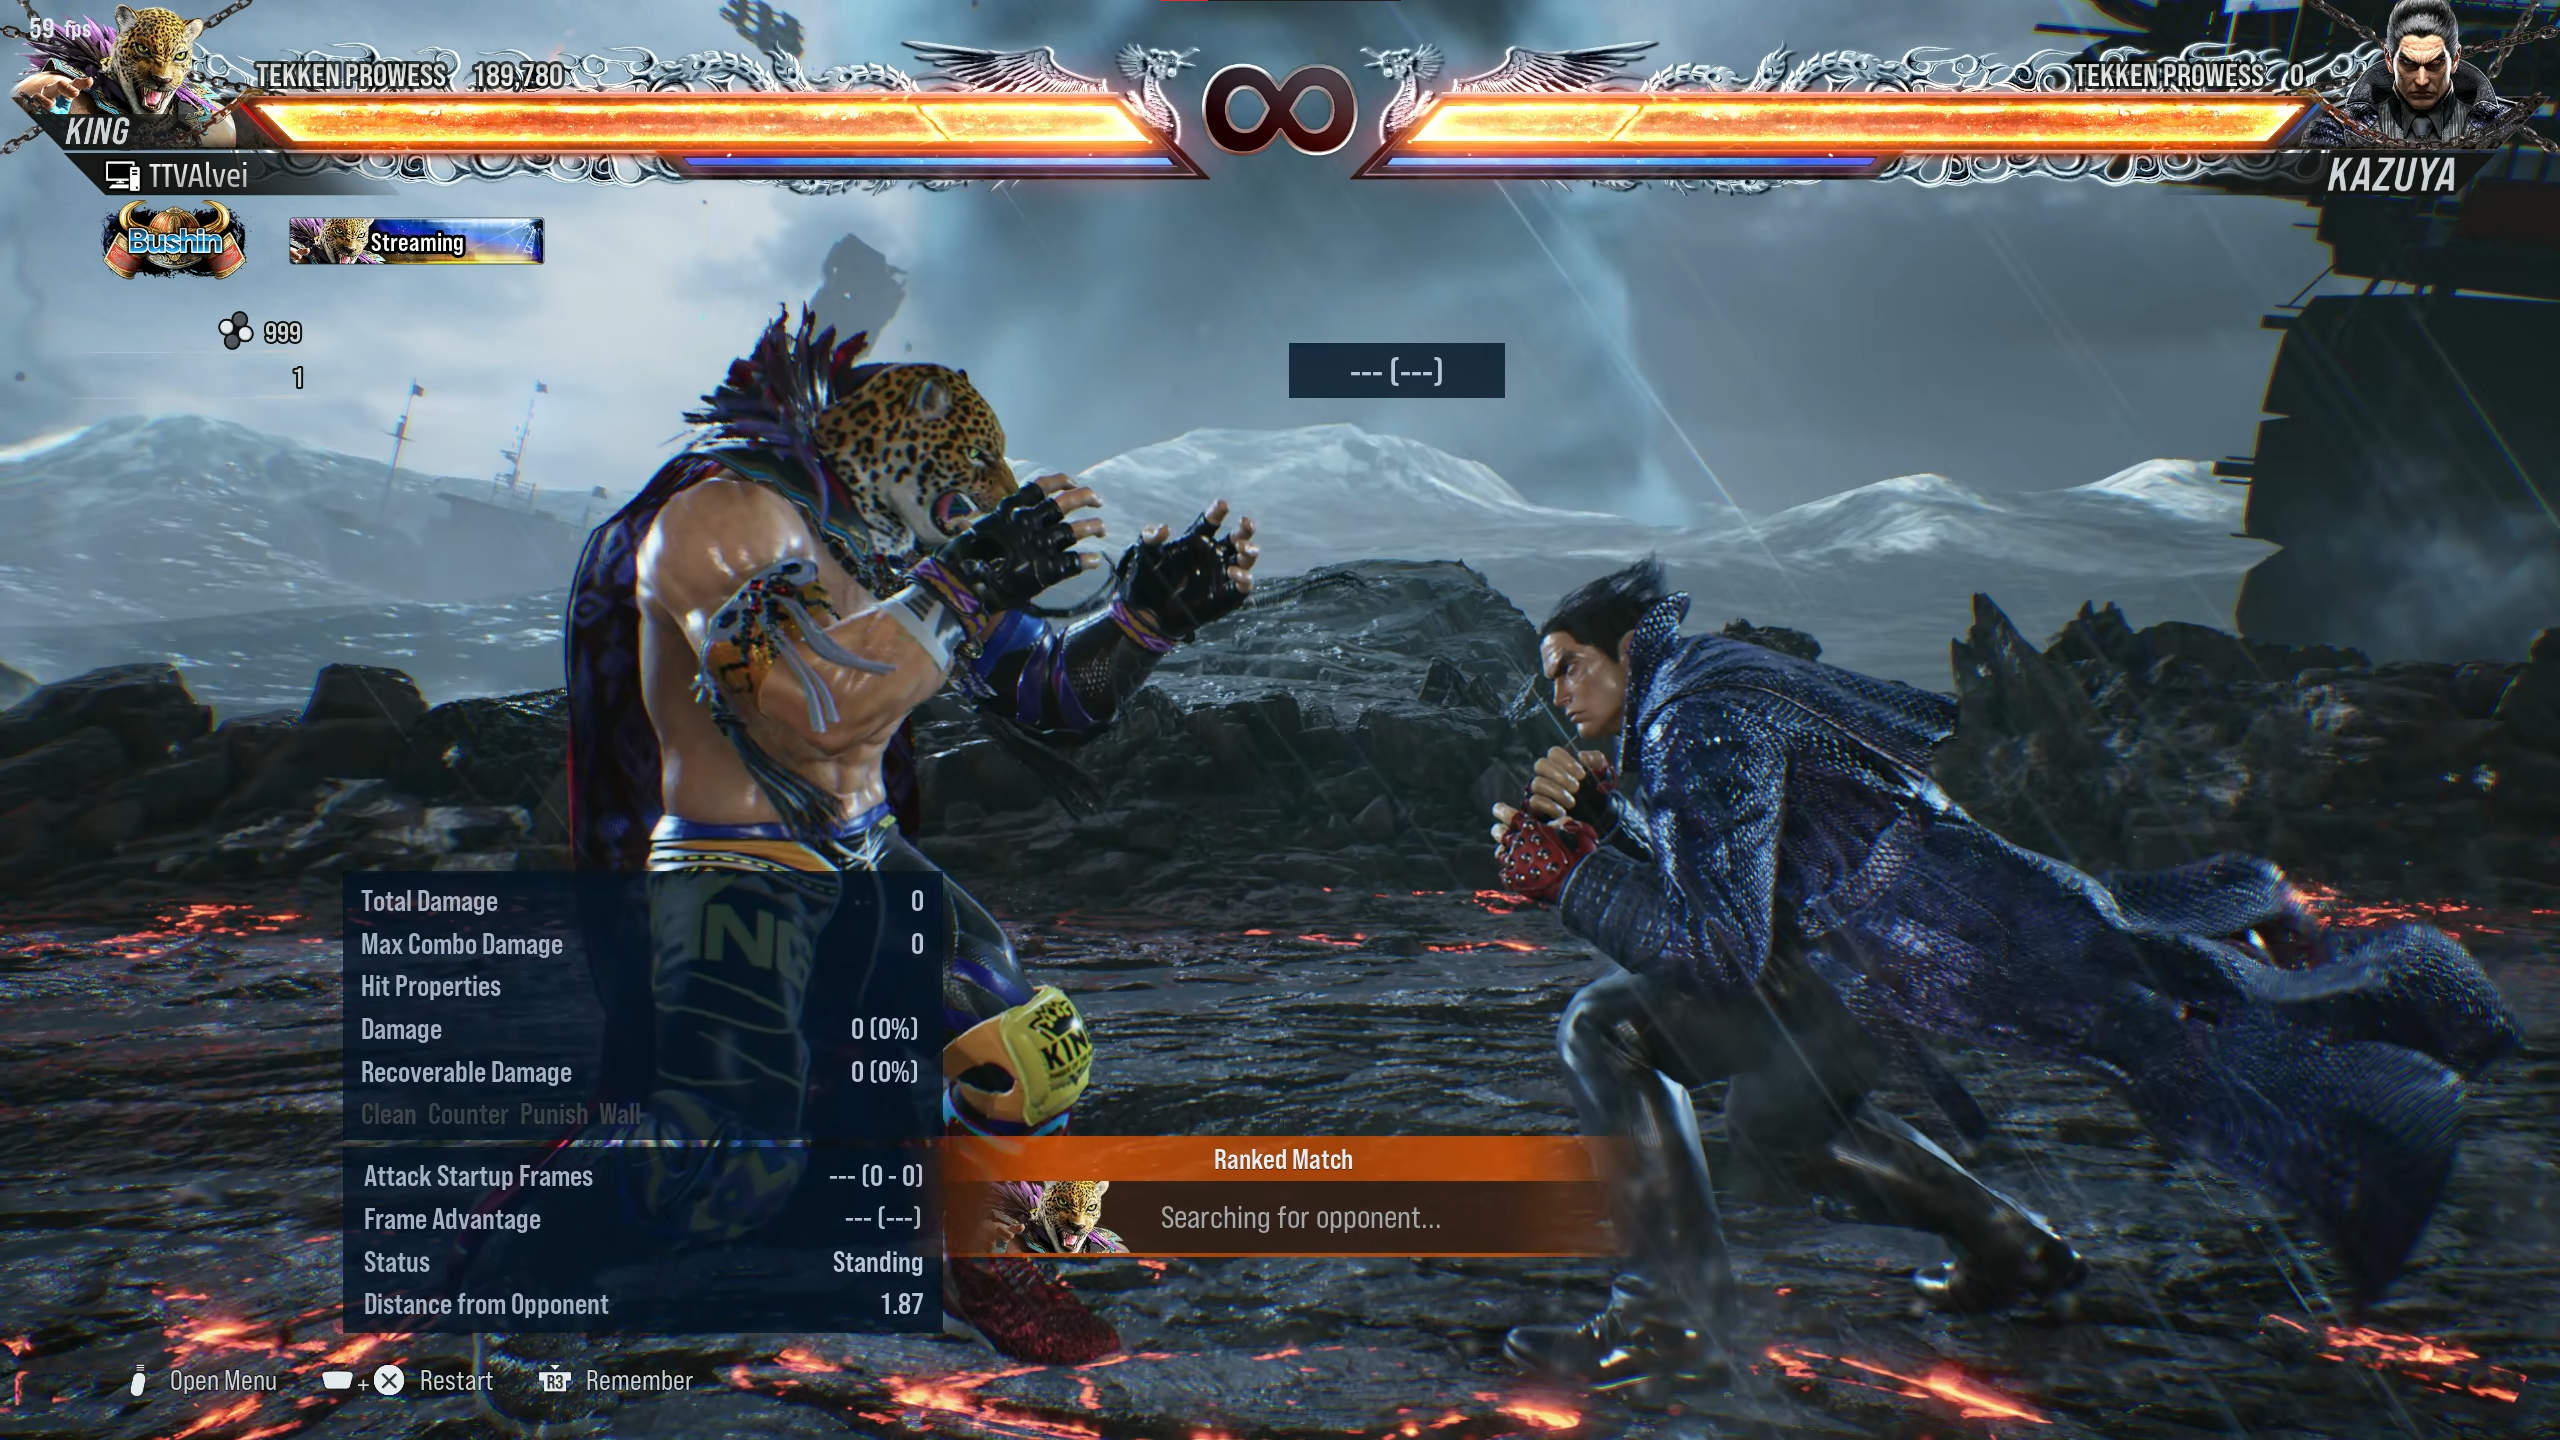
\includegraphics[width=0.48\columnwidth]{../data/TEKKEN/TEKKEN1.png}
\includegraphics[width=0.48\columnwidth]{../data/TEKKEN/TEKKEN1_q25.jpg}
\includegraphics[width=0.48\columnwidth]{../data/TEKKEN/TEKKEN1_q5.jpg}
\includegraphics[width=0.48\columnwidth]{../data/TEKKEN/TEKKEN1_q1.jpg}
\caption{Visual degradation progression for TEKKEN1 screenshot: (top-left) original PNG, (top-right) quality 25, (bottom-left) quality 5, (bottom-right) quality 1. Compression artifacts become increasingly severe, with quality 1 showing extreme blockiness and color distortion.}
\label{fig:visual-degradation}
\end{figure}

\begin{figure}[t]
\centering
\includegraphics[width=\columnwidth]{compression_by_quality.pdf}
\caption{Compression ratio distribution across quality levels for each workflow (generated from \texttt{compress\_images.ipynb}). The figure reveals a clear hierarchy: workflows with highly repetitive content (GIT, TEKKEN) achieve near-maximal compression (96--99\%) even at quality 25, while workflows with varied content (JIRA, EXCEL) require aggressive compression to achieve comparable ratios. GIT maintains consistently high compression across all quality levels, demonstrating that its repetitive patterns (uniform fonts, consistent indentation, repeated UI elements) are so pronounced that moderate quantization suffices. Error bars indicate standard deviation across images within each workflow.}
\label{fig:compression-by-quality}
\end{figure}

\begin{figure}[t]
\centering
\includegraphics[width=\columnwidth]{compression_comparison.pdf}
\caption{Average compression efficiency across workflows (generated from \texttt{compress\_images.ipynb}). The dramatic differences in compression ratios directly reflect the degree of repetitive, structured content: GIT (99.5\%) and TEKKEN (98.2\%) exhibit exceptional compression due to highly repetitive interface elements (code syntax patterns, uniform HUD elements), while JIRA (57.5\%) and EXCEL (44.7\%) show moderate compression due to varied layouts and embedded graphics. This relationship demonstrates that \emph{repetitive data patterns create natural compression opportunities} in screenshot-based workflows (see Section~\ref{subsec:repetitive-patterns}). Error bars indicate standard deviation.}
\label{fig:compression-comparison}
\end{figure}

\section{Conclusion and Future Work}
We presented an empirical study of OCR robustness to JPEG compression in four screen-based workflows and examined how classical feature engineering techniques affect a downstream classifier operating on OCR text. By defining task-specific legibility criteria and varying JPEG quality for each screenshot, we identified compression thresholds beyond which OCR output is no longer reliable for documenting critical user actions. Our compression analysis revealed a fundamental relationship between interface design patterns and compression efficiency: workflows with highly repetitive, structured content (GIT: 99\%+, TEKKEN: 96--98\%) achieve exceptional compression, while those with diverse layouts (JIRA: 40--64\%, EXCEL: 44--67\%) achieve moderate compression. This insight---that \emph{repetitive data patterns create natural compression opportunities}---has practical implications for designing storage-efficient documentation systems that can leverage interface structure to minimize storage requirements without sacrificing OCR accuracy. Using the resulting OCR texts, we compared bag-of-words, filtered, and TF--IDF representations in a logistic regression classifier, finding that reduced and re-weighted feature spaces can match or exceed the performance of a high-dimensional baseline while using fewer effective features.

Future work will extend this framework in several directions. On the vision side, we plan to evaluate multiple OCR engines and explore the impact of additional factors such as resolution scaling and display settings. On the modeling side, we aim to replace manual feature engineering with learned representations, for example by training autoencoders or using pretrained text embeddings on OCR outputs. Ultimately, we envision integrating these components into a full documentation-generation pipeline that couples OCR with large language models, enabling automated, compression-aware capture of complex workflows.

\section*{Acknowledgment}
The author would like to thank the course staff and peers for their feedback on the project design, and acknowledges the use of open-source tools for OCR, data processing, and visualization.

\begin{thebibliography}{00}
\bibitem{b1} R. Smith, ``An overview of the Tesseract OCR engine,'' in \emph{Proc. ICDAR}, 2007, pp. 629--633.
\bibitem{b2} G. Salton and C. Buckley, ``Term-weighting approaches in automatic text retrieval,'' \emph{Information Processing \& Management}, vol. 24, no. 5, pp. 513--523, 1988.
\bibitem{b3} G. E. Hinton and R. R. Salakhutdinov, ``Reducing the dimensionality of data with neural networks,'' \emph{Science}, vol. 313, no. 5786, pp. 504--507, 2006.
\bibitem{b4} Y. LeCun, Y. Bengio, and G. Hinton, ``Deep learning,'' \emph{Nature}, vol. 521, pp. 436--444, 2015.
\bibitem{b5} A. Krizhevsky, I. Sutskever, and G. E. Hinton, ``ImageNet classification with deep convolutional neural networks,'' in \emph{Proc. NIPS}, 2012, pp. 1097--1105.
\bibitem{b6} H. Wei, Y. Sun, and Y. Li, ``DeepSeek-OCR: Contexts Optical Compression,'' \emph{arXiv preprint arXiv:2510.18234}, 2025.
\end{thebibliography}

\end{document}
